\documentclass[12pt, a4paper]{article}

\usepackage[T1]{fontenc}
\usepackage[english]{babel}
\usepackage{mathtools, amsmath, amssymb, amsthm}
\usepackage[hidelinks]{hyperref}
\usepackage{tabularx}
\usepackage{svg}
\usepackage{caption}
\usepackage{float}
\usepackage{booktabs}

\usepackage{tikz}
\usetikzlibrary{arrows.meta, positioning}

\usepackage{minted}
\definecolor{minted_bg}{rgb}{0.9, 0.9, 0.9}
\usemintedstyle{colorful}

\setminted[cpp]{
	tabsize=4,
	% linenos=true,
	bgcolor=minted_bg,
	fontsize=\small,
	mathescape=true
}

\title{Assignment 2\\Collatz Steps}
\author{Federico Bustaffa}
\date{12/03/2025}

\begin{document}

\maketitle
\tableofcontents
\clearpage

\section{Introduction}

The aim of the assignment was to implement, through C++ threads two parallel
versions of an algorithm the computes the \verb|collatz_steps| function on each
value of one or more given ranges.

\begin{minted}{cpp}
  uint64_t collatz_steps(uint64_t n) {
    uint64_t steps = 0;
    while (n != 1) {
      n = (n % 2 == 0) ? n / 2 : 3 * n + 1;
      steps++;
    }

    return steps;
  }
\end{minted}

One implementation has to dispatch the workload through a static policy, in
particular a \emph{block-cyclic} policy, while the other method implement a
dynamic policy like a shared threadpool queue.

In the end a theoretical analysis is performed using the \emph{work-span} model
to estimate the thoretical speedup for both implementations.

\section{Work-Span Analysis}

In order ot reason about the problem with the \emph{work-span} model is
necessary to build a \textbf{dependecy graph}. The chosen approach to compute
the \verb|collatz_steps| function in parallel is to compute one range after the
other but the single range is computed in parallel with a \emph{map-reduce}
pattern.

\begin{figure}[H]
  \centering
  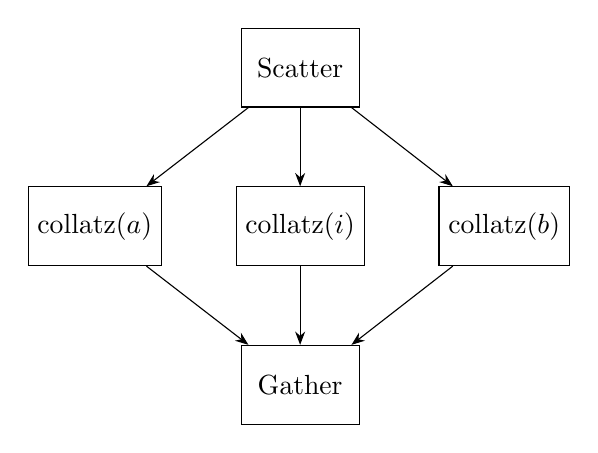
\begin{tikzpicture}[
    node/.style={rectangle, draw, minimum width=1.5cm, minimum height=1cm}, >=Stealth
    ]
    \node[node] (start) {Scatter};
    \node[node, below left=1cm and 1cm of start] (A) {collatz($a$)};
    \node[node, below=1cm of start] (B) {collatz($i$)};
    \node[node, below right=1cm and 1cm of start] (C) {collatz($b$)};
    \node[node, below=1cm of B] (end) {Gather};

    \draw[->] (start) -- (A);
    \draw[->] (start) -- (B);
    \draw[->] (start) -- (C);

    \draw[->] (A) -- (end);
    \draw[->] (B) -- (end);
    \draw[->] (C) -- (end);  
  \end{tikzpicture}
\end{figure}

This kind of graph is very simple to reason about, in fact we can say that the
\textbf{work} $T_1$ is given by the sum of all the task in the graph, assuming
the the average number of steps of the collatz function is $\log{(i)}$.

\[
  T_1 = 1 + \left( \sum_{i=a}^b \text{collatz} (i) \right) + 1
  \approx 1 + \left( \sum_{i=a}^b \log{(i)} \right) + 1 
\]

To simplify a little bit the formula we can make some approximation, using the
assumption that

\[ \text{collatz} (i) \approx  \log{(i)} \]

so 

\[ \text{collatz} (i) < \text{collatz} (i+1) \]

So we can decide to do a quite pessimistic approximation, saying that
$\forall i$ holds $\log{(i)} = \log{(n)}$ where $n = (b-a)+1$. Under these
assumptions we can say that the work can be approximated with

\[ T_1 = 2 + n \cdot \log{(n)} \]

The \text{span} $T_\infty$ is quite trivial to compute, considering that we have
only two levels of dependency and infinite processors, we can easily assume that

\[ T_\infty = 2 + \log (n) \]

The \text{work-span} model tells us that the speedup is limited by the Brent's
theorem and by the minimum between the number of processors $p$ and 
$T_1 / T_\infty$. So in the end we have that

\[
  \frac{p}{1 + p \cdot (T_\infty / T_1)} \leq S(p) \leq
  \min{\left( p, \frac{T_1}{T_\infty} \right)}
\]

If we do some math we have that the speedup lower bound is

\[
  S(p) \geq \frac{p}{1 + p \cdot 
  \left( \frac{2 + \log(n)}{2 + n \cdot \log(n)} \right)} \approx
  \frac{p}{1 + \frac{p}{n}} = \frac{p}{\frac{n + p}{n}} =
  \frac{n \cdot p}{n + p}
\]

For example, considering $p = 16$ and $n = 1.000$ we obtain

\[ S(p) \geq \frac{16 \cdot 1.000}{16 + 1.000} \approx 15.74 \]

and for the upper bound we have

\[
  S(p) \leq = \min{\left( p, \frac{n \cdot \log(n)}{\log(n)} \right)} =
  \min{\left( 16, 10.000 \right)} = 16
\]

As we know and see, the \emph{work-span} model is quite optimistic, due to the
fact that it doesn't take into account parallelization overhead but only the
completion time of each task.

With this highly parallelizable problem is normal that the minimum overhead is
almost equal to the ideal, even for relatively small inputs. This is because the
majority of tasks can be compute indipendently in parallel after satisfying just
one initial dependency.

\section{Static Scheduling}

The first version of the algorithm implements a \emph{block-cyclic} workload
distribution, where ranges are partitioned in blocks and distributed in a round
robin fashion.

For this problem, we don't work on real arrays of data, so there are no problems
like false sharing or cache related problems. We only work on ranges and the
difference in performance among the methods can be explained with the different
distribution of values that are more costly to compute. 

A block-cyclic resulted to be the best option because of the lower overhead for
compute the indices and probably due to the fact that the most coslty values are
better dispatched among threads.

\section{Dynamic Scheduling}

The second version provides a simple implementation of a dynamic scheduling
approach, where all the numbers are enqueued in shared lock-free queue. Each
thread then try to pop a value from the queue and compute the function,
increasing in the end a local counter.

This approach suffers from high overhead of concurrently accessing the queue,
that leads to performance degradation and poor speedup.

\end{document}
